\documentclass{beamer}
\usetheme{Luebeck}
\usecolortheme{beaver}
\setbeamertemplate{navigation symbols}{}

\usepackage{multicol}
\usepackage{cite}
\usepackage[utf8]{inputenc}
\usepackage[ngerman]{babel}
\usepackage{tikz}
\usetikzlibrary{calc}

\definecolor{pbfill}{HTML}{FF6960}% filling color for the progress bar
\definecolor{pbbg}{HTML}{575757}% background color for the progress bar

\makeatletter
\newcommand\progressbar@progressbar{} % the progress bar
\newcount\progressbar@tmpcounta% auxiliary counter
\newcount\progressbar@tmpcountb% auxiliary counter
\newdimen\progressbar@pbht %progressbar height
\newdimen\progressbar@pbwd %progressbar width
\newdimen\progressbar@tmpdim % auxiliary dimension

\progressbar@pbwd=\paperwidth
\progressbar@pbht=0.5ex
\newcommand\progressbar@ffn{1}% Anzahl frames für Titelseite und 


% add page numbering
\expandafter\def\expandafter\insertshorttitle\expandafter{%
	\insertshorttitle\hfill%
	\hspace{100px}\insertframenumber\,/\,\inserttotalframenumber}

% the progress bar
\def\progressbar@progressbar{%
	\ifnum\insertframenumber>\progressbar@ffn
	
	\progressbar@tmpcounta=\insertframenumber
	\advance\progressbar@tmpcounta by -\progressbar@ffn
	\progressbar@tmpcountb=\inserttotalframenumber
	\advance\progressbar@tmpcountb by -\progressbar@ffn
	\progressbar@tmpdim=\progressbar@pbwd
	\multiply\progressbar@tmpdim by \progressbar@tmpcounta
	\divide\progressbar@tmpdim by \progressbar@tmpcountb
	
	\begin{tikzpicture}
		
	%%\shade[top color=pbbg!20,bottom color=pbbg!20,middle color=pbbg!20]
	\path[fill=pbbg!20]
	(0pt, 0pt) rectangle ++ (\progressbar@pbwd, \progressbar@pbht);
	
	%%\shade[draw=pbfill,top color=pbfill!50,bottom color=pbfill!50,middle color=pbfill] 
	\path[fill=pbfill!70]
	(0pt, 0pt) rectangle ++ (\progressbar@tmpdim, \progressbar@pbht);
	
	\end{tikzpicture}%
	\fi%
}

\addtobeamertemplate{footline}
{%
	\begin{beamercolorbox}[wd=\paperwidth,ht=3ex,center,dp=0ex]{white}%
		\progressbar@progressbar%
	\end{beamercolorbox}%
}{}
\makeatother
%#####


\title{Partikelsensoren}
\author{Steffen Walter (1145690)}
\institute{Duale Hochschule Baden-Württemberg -- Stuttgart\newline Vorlesung: Sensorik und Aktorik}
\centering
\date{31. März 2019}
\begin{document}
	\maketitle
	\begin{frame}{Agenda}
		\section{Agenda}
		\begin{enumerate}
			\item Anwendungen
			\item Messtechniken
			\begin{itemize}
				\item Resistive Messung
				\item Extinktionsmessung
				\item Streulichtmessung
				\item Laserbeugung
			\end{itemize}
			\item Fazit
		\end{enumerate}
	\end{frame}

	
	\begin{frame}{Anwendungen}
	\framesubtitle{Wo in der Praxis werden Partikelsensoren benötigt?}
	\section{Anwendungen}
	\begin{itemize}
		\item Gase
		\begin{itemize}
			\item Abgassystem
			\item Reinraumüberwachung
			\item Luftqualitätsüberwachung
		\end{itemize}
		\item Flüssigkeiten
		\begin{itemize}
			\item Leistungsmessung Filter
			\item Hydrauliksystemüberwachung
			\item Wasserqualitätsüberwachung
			\item Medizintechnik: Reinheit von Injektionslösungen
		\end{itemize}
	\end{itemize}
	\end{frame}

	\begin{frame}{Messtechniken}
	\framesubtitle{Welche verschieden Techniken werden zur Erfassung von Parktikeln verwendet?}
	\section{Messtechniken}
		\begin{itemize}
			\item Resistives Verfahren
			\item Optische Verfahren	
			\begin{itemize}
				\item Extinktionsmessung
				\item Streulichtmessung
				\item Laserbeugung
			\end{itemize}
		\end{itemize}
	\end{frame}
	
	\begin{frame}{Resistives Verfahren}
		\begin{block}{Aufbau}
			Das Sensorelement besteht aus einer Interdigitalstruktur mit zwei kammförmigen Elektroden aus Platin auf einem keramischen Substrat mit einem integrierten Heizelement. Ein Platinmäander dient zur Messung der Temperatur des Sensorelements.
		\end{block}
		\begin{multicols}{2}
		\footnotesize{
		\begin{itemize}
			\item Anwendung im Abgassystem von Autos 
			\item Notwendigkeit durch On-Board-Diagnose-Bestimmungen von Dieselpartikelfiltern
			\item Messung der Rußemission nach dem Partikelfilter.
		\end{itemize}
		\begin{figure}
			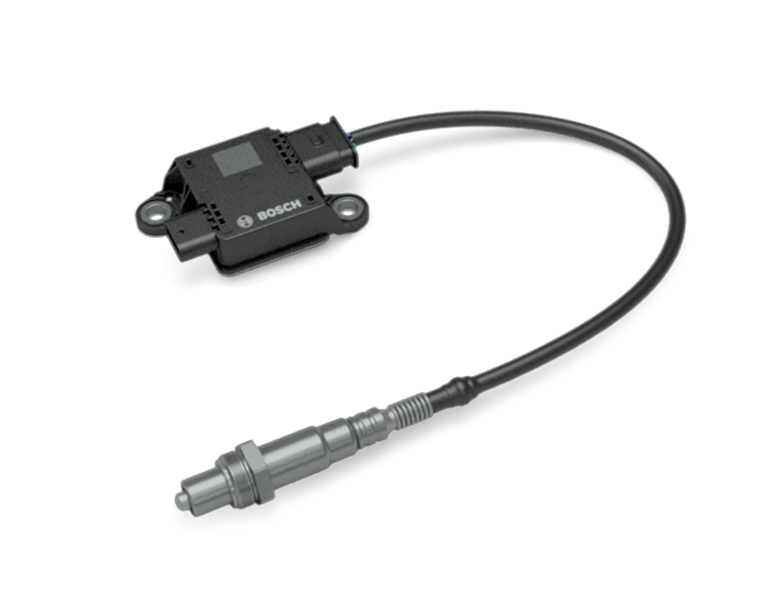
\includegraphics[width=0.35\textheight]{russ.png}
			\caption{\footnotesize Partikelsensor für Abgassystem. Quelle\cite{bosch}}
		\end{figure}}
		\end{multicols}
	\end{frame}

	\begin{frame}{Resistives Verfahren}
	\begin{multicols}{2}
		\footnotesize{
			\begin{enumerate}
				\item Anfangs sehr hoher Widerstand
				\item Spannung wirkt anziehend auf Rußpartikel
				\item Partikel bilden leitfähige Rußpfade
				\item Monoton fallende Widerstandskurve
				\item Ende der Messung bei Schwellwert
				\item Rücksetzung und Regeneration durch Verbrennung der Ablagerungen
		\end{enumerate}}
		\begin{figure}
			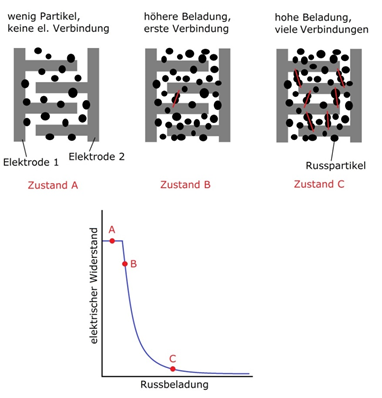
\includegraphics[width=0.6\textheight]{russ_kurve.png}
			\caption{\footnotesize Funktionsweise eines resistiven Rußsensor. Quelle\cite{mtec}}
		\end{figure}
	\end{multicols}
	\end{frame}	

	\begin{frame}{Resistives Verfahren}
	\begin{multicols}{2}
		\begin{enumerate}
			\item Abgas
			\item Interdigitalstruktur
			\item Keramik
			\item Isolation
			\item Heizelement
			\item Platinmäander
		\end{enumerate}
		\begin{figure}
			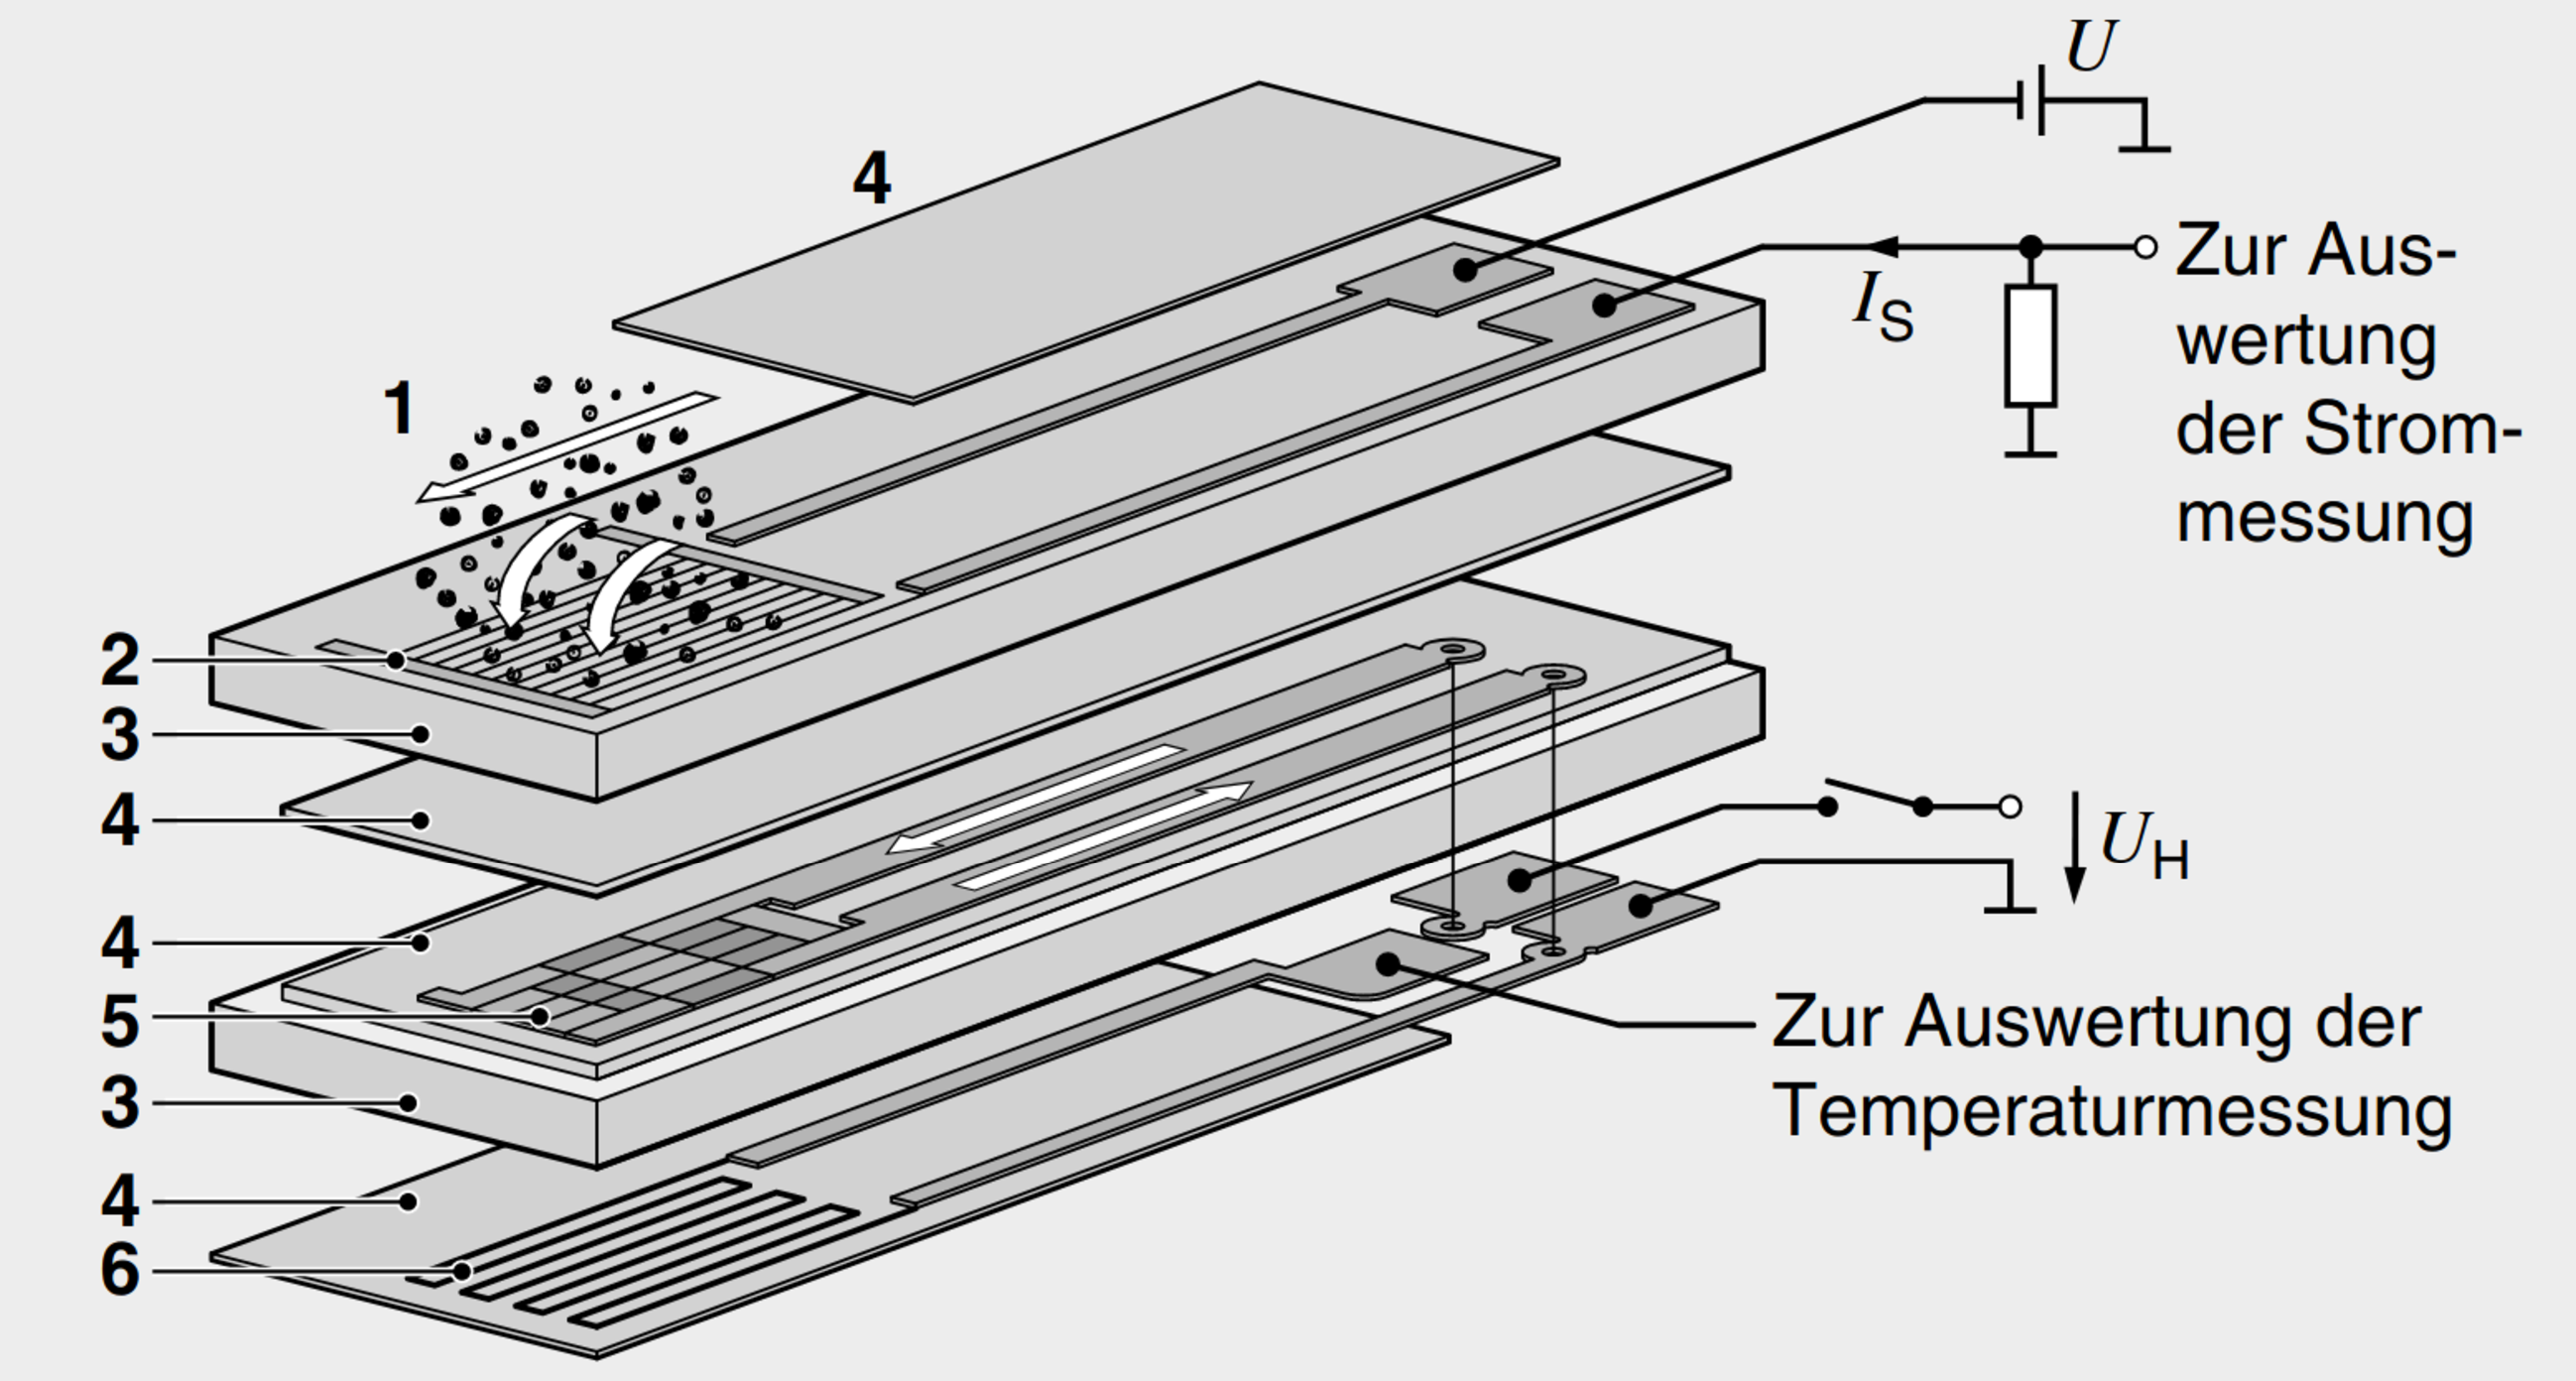
\includegraphics[width=0.75\textheight]{feld.pdf}
			\caption{\footnotesize{Explosionszeichnung des Sensors. Quelle\cite{feld}}}
		\end{figure}
	\end{multicols}
	\end{frame}

	\begin{frame}{Extinktionsmessung}
		\begin{block}{Funktionsweise}
			\footnotesize Bei der Extinktionsmessung wird die Reduktion der Lichtintensität eines Lichtstrahls beim Durchgang einer Flüssigkeit gemessen. Je mehr Partikel sich im Testobjekt befinden, desto größer ist die Abschwächung.
			\begin{figure}
				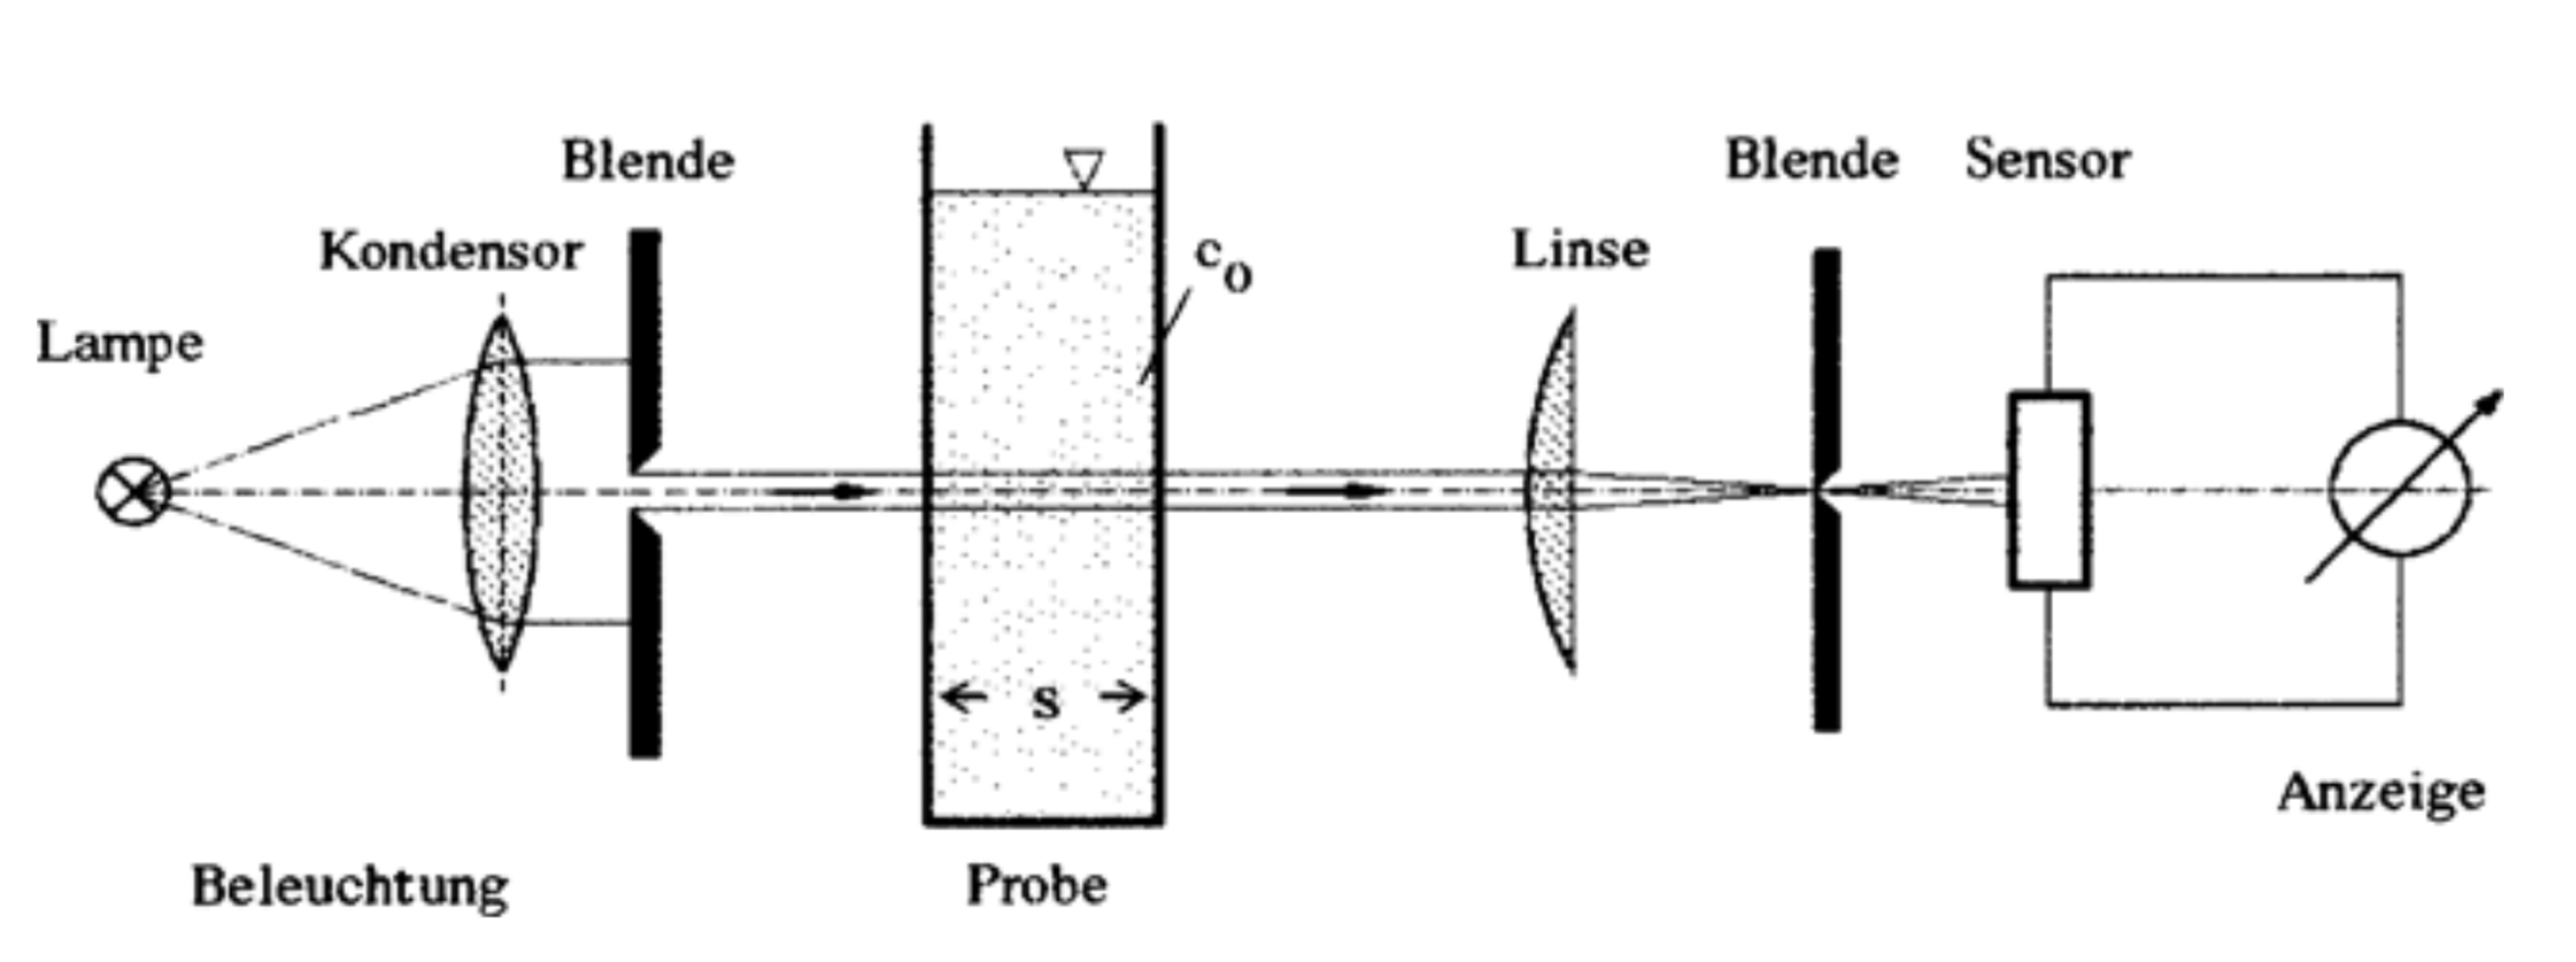
\includegraphics[width=\textheight]{extinktion.pdf}
				\caption{\footnotesize{Fotometrische Extinktionsmessung. Quelle\cite{messtechniken}}}
			\end{figure}
		\end{block}
	\end{frame}

	\begin{frame}{Streulichtmessung}
		\begin{block}{Funktionsweise}
			\begin{multicols}{2}
				\footnotesize Bei der Streulichtmessung wird eine parallele Lichtquelle herangezogen.
				Trifft das Licht auf einen Partikel, kommt es zur Streuung des Lichtes. Eintretende Effekte sind Beugung, Brechung und Reflexion.
				Die Erfassung der Streulicht-Intensitätsverteilung kann auf die Größe des erfassten Partikels rückgeschlossen werden.
				\begin{figure}
					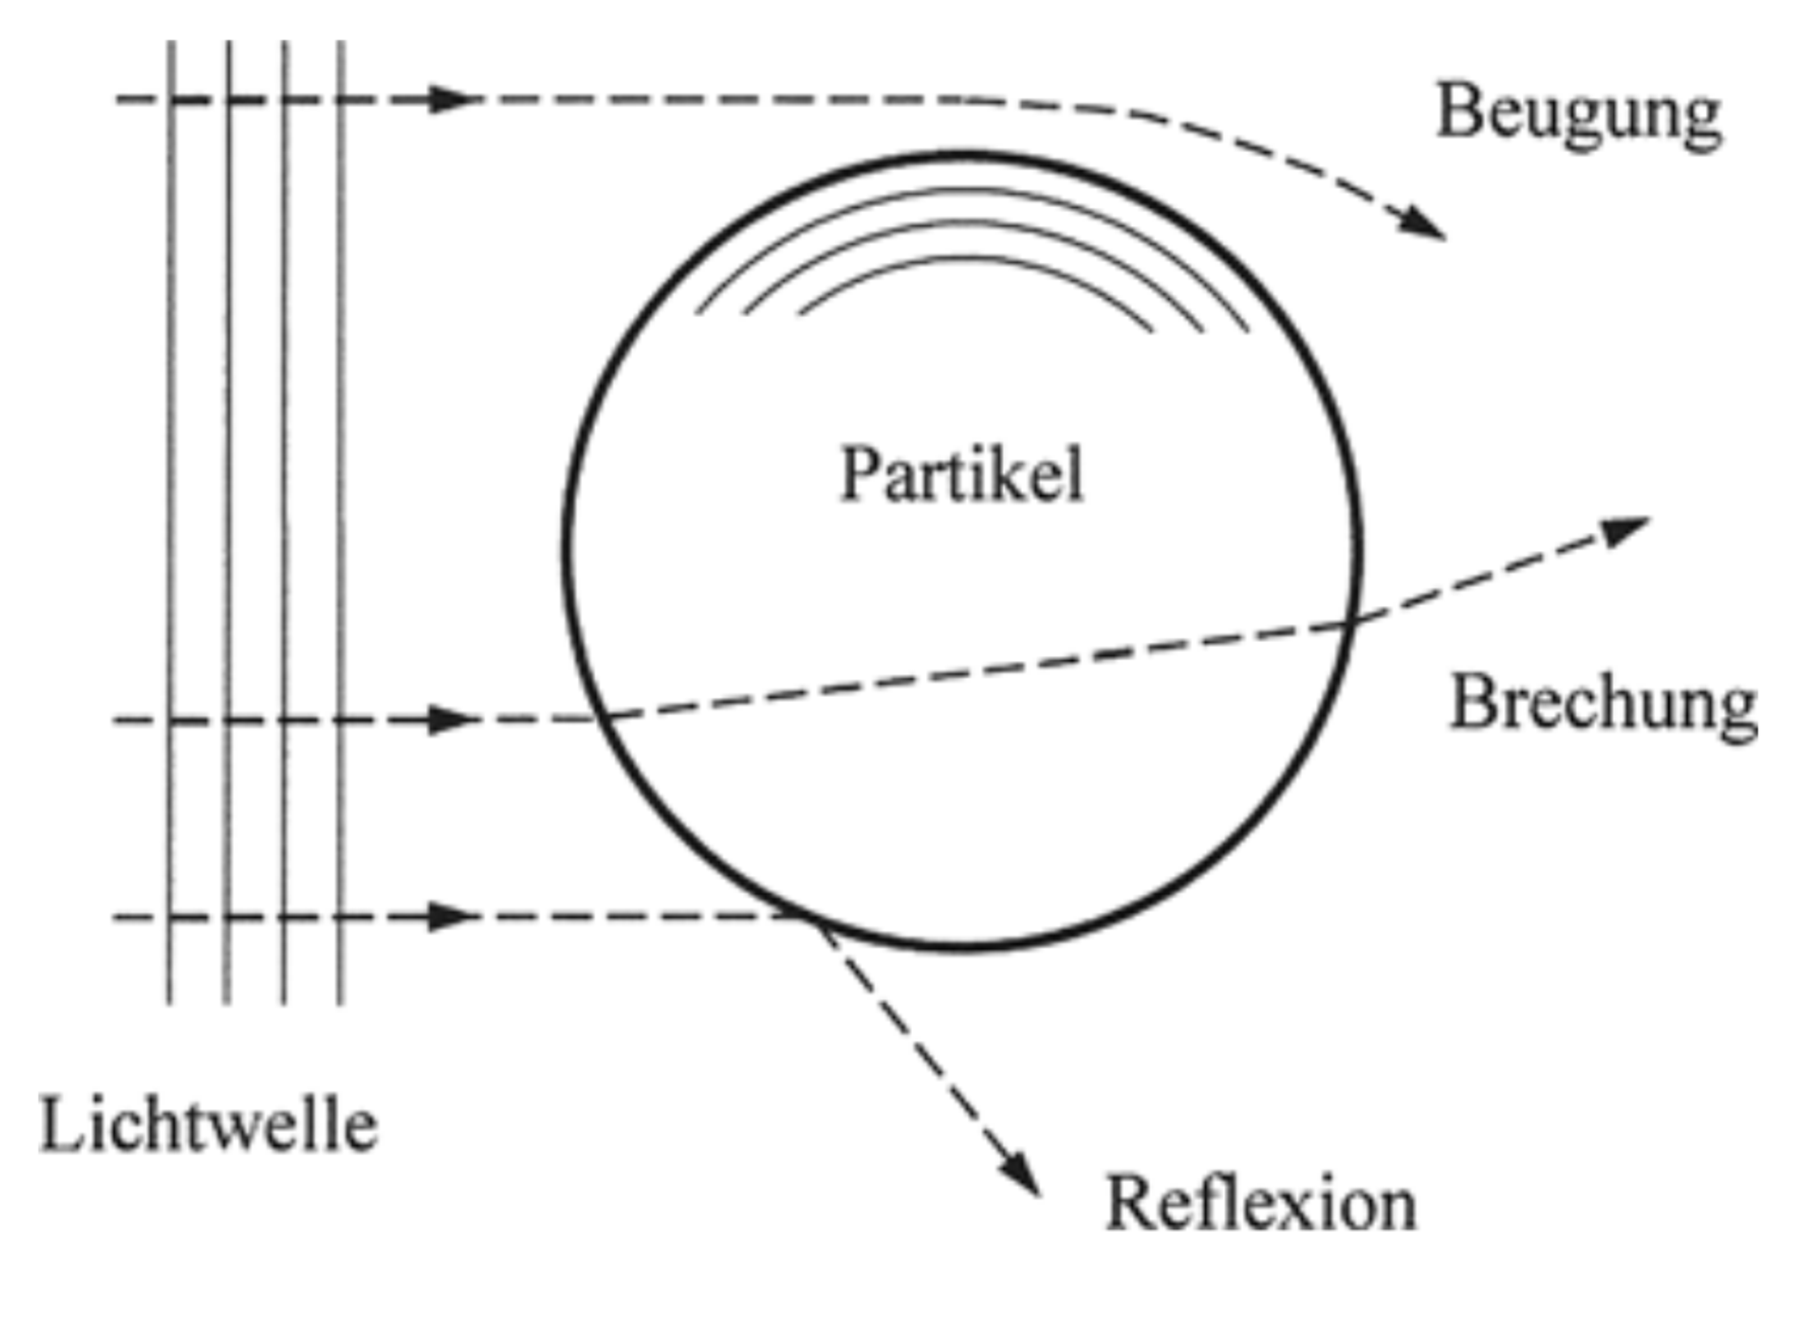
\includegraphics[width=0.6\textheight]{streulicht.pdf}
					\caption{\footnotesize{Streuung an einem einzelnen Partikel. Quelle\cite{messtechniken}}}
				\end{figure}
			\end{multicols}
		\end{block}
	\end{frame}

	\begin{frame}{Streulichtmessung an Partikelkollektiven (Laserbeugung)}	
		\begin{block}{Funktionsweise}
			\footnotesize Bei Anwendung der Streulichtmessung auf einen mit Partikeln durchsetzten Raum und der nachgelagerten Weiterverarbeitung durch eine Linse, entsteht eine abweichendes Beugungsspektrum auf einer Projektionsfläche. Durch die Auswertung der verschieden Beugungsspektren ist kann mathematisch auf Anzahl und Größe der Partikel rückgeschlossen werden.
			\begin{figure}
				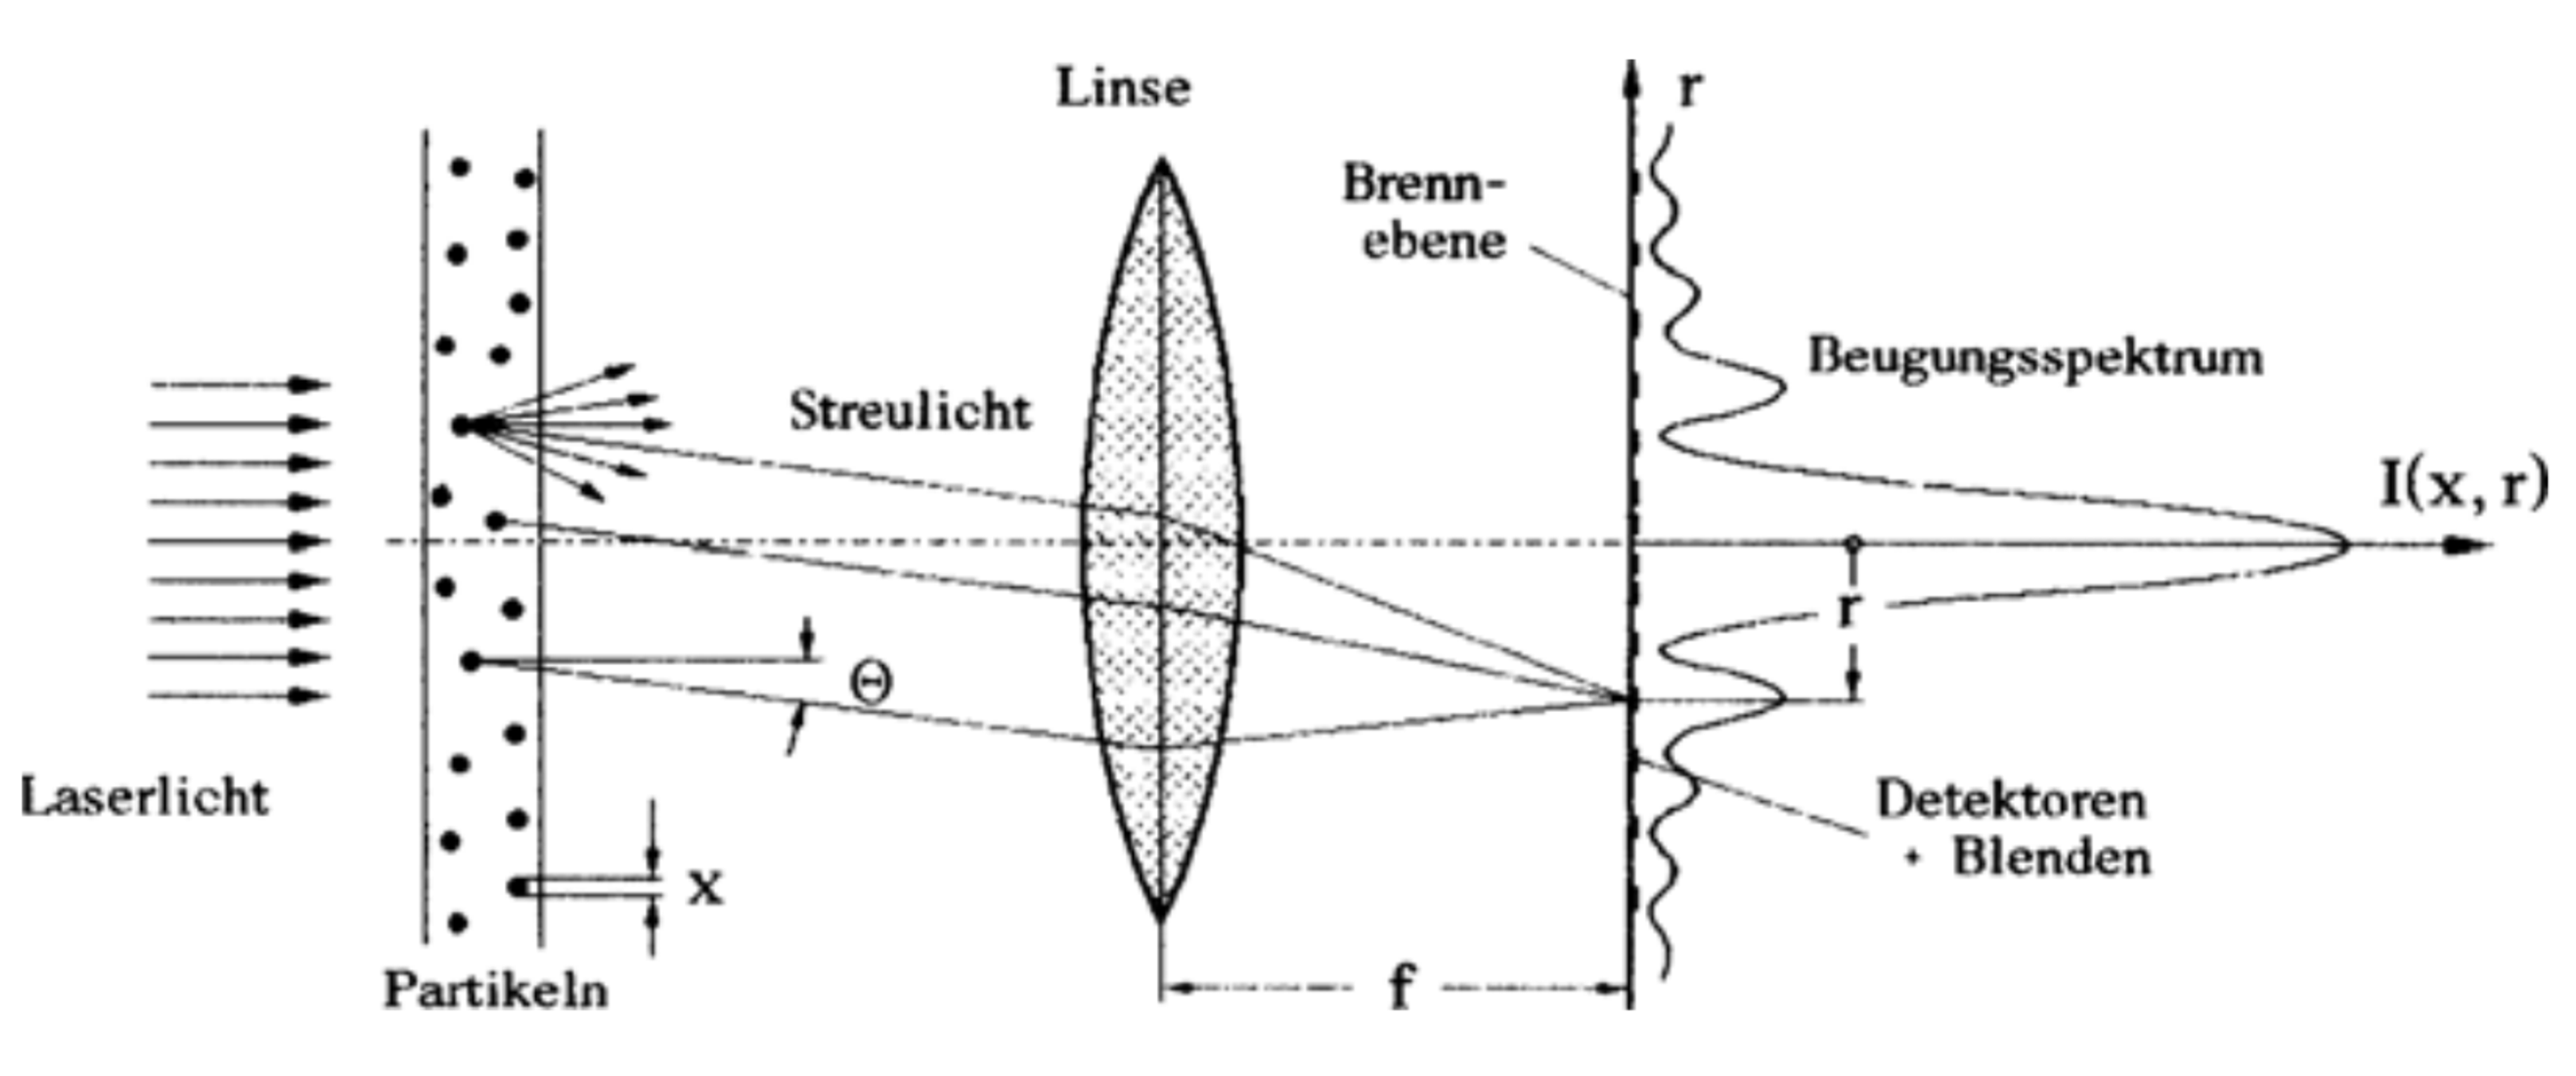
\includegraphics[width=0.8\textheight]{laser.pdf}
				\caption{\footnotesize{Streuung an einem Partikelkollektiv. Quelle\cite{messtechniken}}}
			\end{figure}
		\end{block}
	\end{frame}

	\begin{frame}{Fazit}
	\section{Fazit}
	\begin{itemize}
		\item Viele Unterschiedliche Methoden
		\item Stark abhängig von der Anwendungsfall
		\item Maßstäbe zur Auswahl:
		\begin{itemize}
			\item Partikelgröße
			\item Spezielle Materialeigenschaften
			\item Gewünschte Information (Größe, Dichte)
			\item Präzision
		\end{itemize}
	\end{itemize}
	\end{frame}
	
	\begin{frame}{Quellen}
		\begin{multicols}{2}
		\tiny{
			\bibliographystyle{plainnat}
			\bibliography{literatur}
		}
		\end{multicols}
	\end{frame}
	
\end{document}